\section{Eine IDE f{\"u}r daten- und performancebewusste Entwicklung}\label{chap:entwicklungsumgebung}

%%%%%%%%%%%%%%%%
%
%   Eine IDE für daten- und performancebewusste Software-Entwicklung
%
%%%%%%%%%%%%%%%%

\begin{figure}[ht]
	\centering
  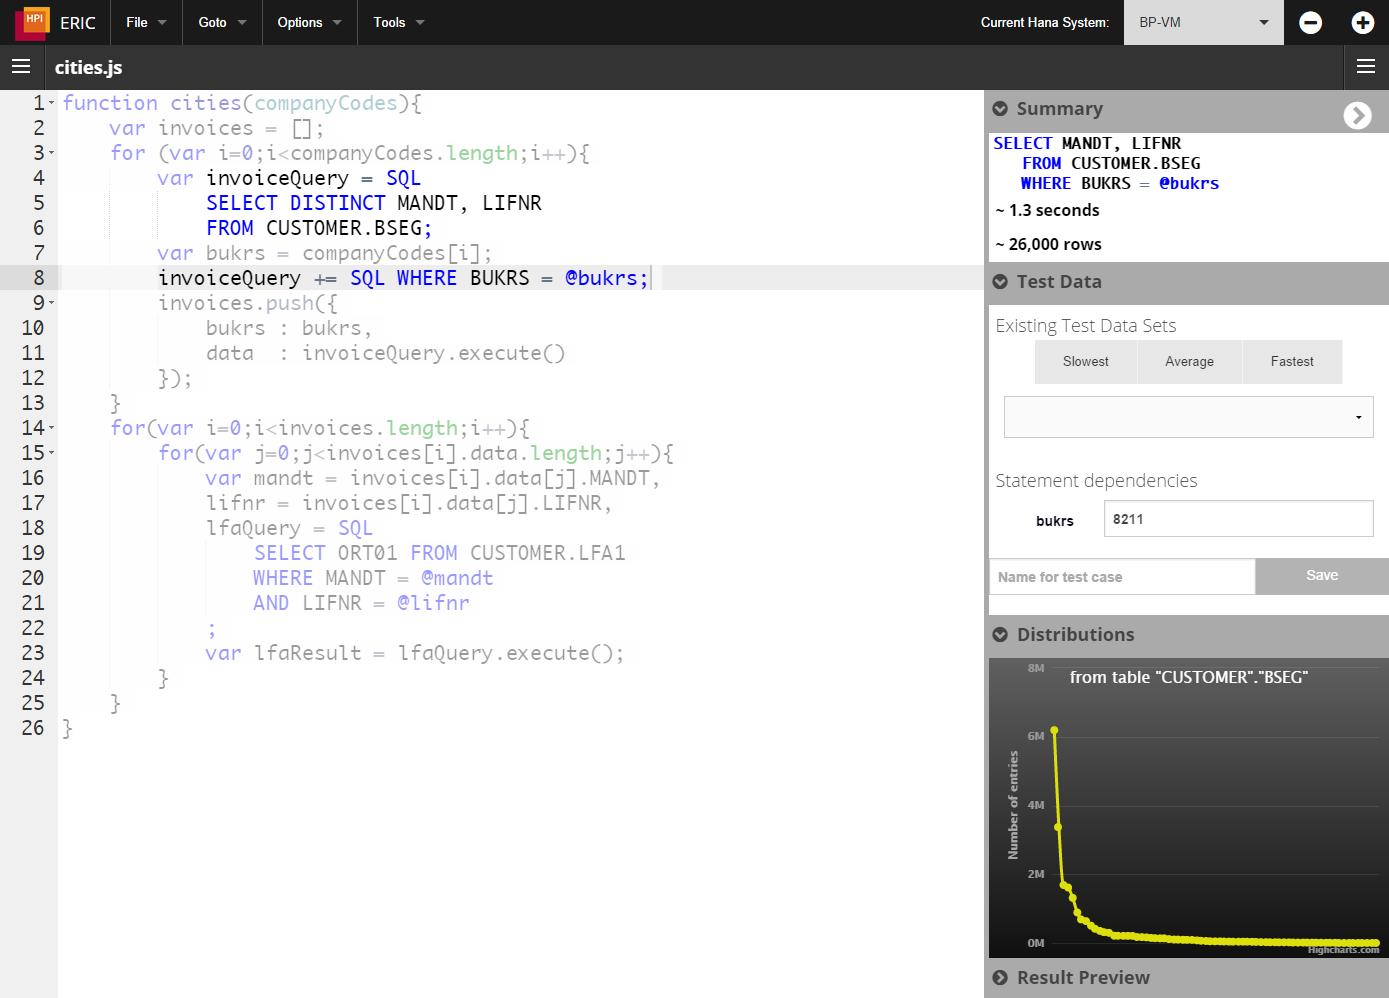
\includegraphics[width=0.94\textwidth]{figures/ide.png}
	\caption{Übersicht der Web IDE}
	\label{fig:ide}
\end{figure}

Die im Rahmen des Bachelorprojektes ``Modern Computer-Aided Software Engineering'' entwickelte Web IDE (Abbildung \ref{fig:ide}) vereint eine Reihe von Konzepten zur Entwicklung von Geschäftsanwendungen mit dem Fokus auf der besseren Integration von Informationen aus Datenbanken.
Besonders die Schärfung des Bewusstseins für Daten und Datenmengen sowie das vorausschauende Entwickeln in Hinblick auf die Skalierung der Anwendung soll gefördert werden.
Grundlage dafür bietet die Einbettung von SQL in die Programmiersprache der Geschäftsanwendung \cite{Horschig2014} (mehr Details dazu in Kapitel \ref{sec:dependencydetection}).
Durch das Parsen des Quelltextes und der darin enthaltenen SQL-Statements \cite{Schulz2014} werden die Voraussetzungen geschaffen, Analysen und Visualisierungen der Datenabfragen durchzuführen.
Unter anderem kann anschließend eine Abschätzung über die Laufzeiten und Ergebnisgrößen von SQL-Statements gegeben werden, sowie eine Vorschau der Ergebnisse und die Verteilung der Daten in den angefragten Spalten.
Für die Berechnung der abgeschätzten Laufzeiten und Ergebnisgrößen stehen zwei Verfahren zur Auswahl: auf Basis von Sampling \cite{Exner2014} werden mithilfe von Teilmengen der Relationen ungefähre Größen hochgerechnet und durch den Ansatz des Machine Learnings \cite{Mues2014} können Ergebnisse vergangener Anfragen als Grundlage der Berechnung genutzt werden.

\begin{figure}[ht]
	\centering
  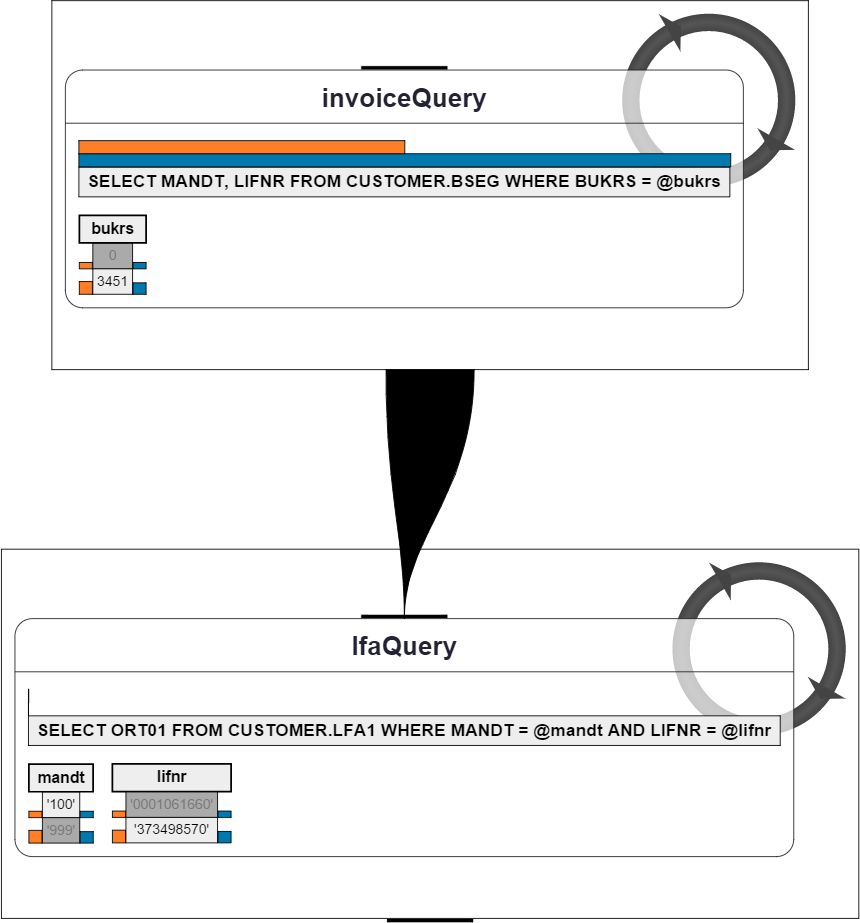
\includegraphics[width=0.3\textwidth]{figures/feedback.png}
	\caption{Visualisierung des Kontrollflusses}
	\label{fig:feedback}
\end{figure}

Zusätzlich ist es möglich den Verlauf des Kontrollflusses in Zusammenhang mit den Datenanfragen als Visualisierung zu betrachten \cite{Frahnow2014} (zu sehen in Abbildung \ref{fig:feedback}) um die Ursachen von Performance-Problemen ausfindig zu machen.

Die betrachteten Features für die Analysen von SQL-Statements haben dabei zwei Voraussetzungen: das SQL-Statement muss komplett erfasst und dessen variable Parameter müssen testweise mit Werten belegt sein.

\begin{lstlisting}[caption={Variablen nehmen Einfluss auf die SQL-Query und -Parameter}, label={lst:ide}, language=JavaScript]
	var firstname = request.body.firstname;
	var country = request.body.country;
	var stmt = ``SELECT * FROM WorldPopulation WHERE country = '';
	if(country == ``D''){
		stmt += ``Germany'';
	} else {
		stmt += ``China'';
	}
	if(firstname){
		stmt += `` AND firstname = `` firstname;
	}
\end{lstlisting}

Schon einfache Algorithmen, wie im Code-Beispiel \ref{lst:ide}, lassen das SQL-Statement auf Basis von Programmvariablen variieren (\texttt{country}) und belegen die SQL-Parameter in Abhängigkeit von zum Beispiel Session-Daten, Formularen oder Anfrage-Parametern mit unterschiedlichen Werten (\texttt{firstname}).
Dadurch ist es für den Entwickler schwer abzuschätzen, welche Werte repräsentativ sind oder sogar Randfälle darstellen und die Antwortzeit der Anwendung in die Höhe treiben.
Deshalb ist es wichtig sinnvolle Testwerte und Kombinationen von Testwerten zu nutzen, die die verschiedenen Szenarien innerhalb der Anwendung abdecken.
Mit der Theorie und möglichen Algorithmen zum Vorschlagen dieser Daten beschäftigt sich diese Bachelorarbeit und diskutiert sie in den folgenden Kapiteln.
